\newpage
\section{Konzeptfindung}

Das Endziel ist ein möglichst einfaches und zuverlässiges Gesamtkonzept, welches möglichst robust und Fehler-unanfällig funktioniert. Dies möchten wir erreichen, in dem wir vorgängig alle Lösungsansätze aus der Technologierecherche, welche mit grossen Risiken verbunden sind, erkennen und ausscheiden. Mit den verbleibenden Ansätzen wird ein Morphologischer-Kasten erstellt, um ein Gesamtkonzept zu entwickeln. Um mit dem Morphologischen Kasten die optimale Variante zu finden, wird zu einigen Teilfunktionen des Fahrzeuges eine Nutzwertanalyse erstellt.

\subsection{Vorauswahl}
    \subsubsection{Fortbewegung}
        Da das Fahrzeug in der Lage sein muss, sich an Ort und Stelle um die eigene Achse zu wenden, sind die Optionen Knicklenkung, Achsschenkellenkung und Drehschemellenkung nicht geeignet.
        Das Prinzip 'Fahrzeug ab bocken und drehen' ist als alleiniges Lenksystem ungeeignet, weil es zu viel Zeit benötigt für das Lenkmanöver. Es wird als optionalen Plan-B beibehalten für den Fall, dass das Fahrzeug beim Wenden während dem Hindernishandling verrutscht. Falls dieses Problem beim Testen auftritt, kann das System nachgerüstet werden.
        Omniwheels und Mecanum-Räder sind sehr ähnlich, nur die Form und Anordnung der Rollen auf den Rädern ist unterschiedlich. Bei Omniwheels sind die Rollen in einem Winkel von 90° an den Rädern befestigt, wobei sie bei Mecanum-Rädern in 45° angeordnet sind und eine Tonnenform aufweisen. Dadurch versprechen die Mecanum-Räder eine geringere Anfälligkeit, sich in den Plattenfugen zu verfangen. Die 4-Rad Differential Lenkung und das Prinzip Roomba sind von der Wendigkeit und dem konstruktiven Aufwand vergleichbar, jedoch besteht bei der 4-Rad Variante die Gefahr von Aufschaukeln bei einer Drehung an Ort und Stelle, sowie die Gefahr von Schieben der langsameren Rädern bei Kurvenfahrt.

        \subparagraph{Nutzwertanalyse Fortbewegung}
        Damit eine genauere Analyse zwischen Mecanum-Rädern und dem Prinzip Roomba durchgeführt werden kann, wird eine Nutzwertanalyse durchgeführt. der Gewinner ist das Prinzip Roomba (ersichtlich in folgender Tabelle).
        

        
    \newpage
    \subsubsection{Hindernis Bewältigung}
        \paragraph{Aufnahme}
            Da das Konzept möglichst einfach und zuverlässig gestaltet werden soll, scheiden die Ideen 'Gabelstapler' und 'Vakuumgreifer' aus der Vorauswahl aus. Der Gabelstapler erfordert eine äusserst präzise und aufwendige Sensorik, um die Löcher für die Aufnahme genau zu treffen. Der Vakuumgreifer wiederum zeigt im Vergleich zu den 'Klemmen' eine geringere Zuverlässigkeit. Um eine vergleichbare Zuverlässigkeit zu erreichen, wären umfangreiche Tests erforderlich, ohne dass der Vakuumgreifer dabei signifikante Vorteile gegenüber den 'Klemmen' bieten würde.

        \subparagraph{Nutzwertanalyse Aufnahme}
        Damit eine genauere Analyse zwischen Klemme Breitenweg und Klemme Längsweg durchgeführt werden konnte, wurde eine Nutzwertanalyse durchgeführt. Der Gewinner war dank der höheren Präzision Klemme Breitenweg, was auch in Tabelle \ref{tab:konzept_nutzwertanalyse_aufnahme} ersichtlich ist.
        
        \begin{table}[H]
        \resizebox{\textwidth}{!}{
         \centering
         \renewcommand{\arraystretch}{1.5}
             \begin{tabular}{|c|>{\raggedright} p{3cm}|c|c|c|>{\raggedright} p{3cm}|c|c|>{\raggedright\arraybackslash}p{3cm}|}
                \hline
                \multicolumn{3}{|c|}{} & \multicolumn{3}{c|}{\textbf{Klemme Breitenweg}} & \multicolumn{3}{c|}{\textbf{Klemme Längsweg}} \\ \hline
                \textbf{Kriterium} & \textbf{Erklärung} & \textbf{Gewichtung} & \textbf{Bewertung} & \textbf{Punkte} & \textbf{Begründung} & \textbf{Bewertung} & \textbf{Punkte} & \textbf{Begründung} \\ \hline
                Sicherer Halt & Wie gut hält das Hindernis in der Halterung & 35 & 7 & 245 & Relativ starke Punktlast, aber dennoch sehr guter Halt & 8 & 280 & Große Fläche zur Kraftübertragung, stabil und sehr guter Halt \\ \hline
                Präzision & Wie präzise ist die Vorrichtung, auch wenn das Fahrzeug nicht genau zentriert vor dem Hindernis steht & 30 & 7 & 210 & Siehe Kapitel Präzision, detaillierte Erklärung & 4 & 120 & Siehe Kapitel Präzision, detaillierte Erklärung \\ \hline
                Komplexität & Wie aufwendig ist die Konstruktion & 20 & 5 & 100 & Nicht sehr komplex & 5 & 100 & Nicht sehr komplex \\ \hline
                Kosten & Wie viel kostet die Vorrichtung & 15 & 4 & 60 & 3D-Druck möglich & 4 & 60 & 3D-Druck möglich \\ \hline
                \multicolumn{2}{|r|}{\textbf{Nutzwert:}} & 100 & & 615 & & & 560 & \\ \hline
            \end{tabular}
         }
            \caption{Nutzwertanalyse Hinderniss Aufnahme}
            \label{tab:konzept_nutzwertanalyse_aufnahme}
        \end{table}

        \newpage
            
            \subparagraph{Präzision}

            In der Nutzwertanalyse wird erwähnt, dass das Kriterium Präzision eine genauere Erklärung benötigt. Die Präzision der Klemme Breitenweg kann besser erreicht werden als bei der Klemme Längsweg. Einerseits kann, wie in den Abbildungen \ref{img:konzept_zentrierung_1} und \ref{img:konzept_zentrierung_2} gezeigt, eine Zentrierung bei der Klemme Breitenweg eingebaut werden. Diese Zentrierung fehlt bei der Klemme Längsweg. Da unter anderem das Ziel ist, das Hindernis möglichst zentriert wieder auf dem Klebeband abzustellen, verliert hier die Klemme Längsweg an Punkten. In Abbildung \ref{img:konzept_zentrierung_3} wird dargestellt, dass, wenn das Fahrzeug nicht perfekt mittig auf das Hindernis zufährt, automatisch ein Fehler generiert wird, weil das 'Offset' nicht, ohne komplexere Sensorik, miteinbezogen werden kann.


            \begin{figure}[h!]
                \centering
                \begin{minipage}{0.48\textwidth}
                    \centering
                    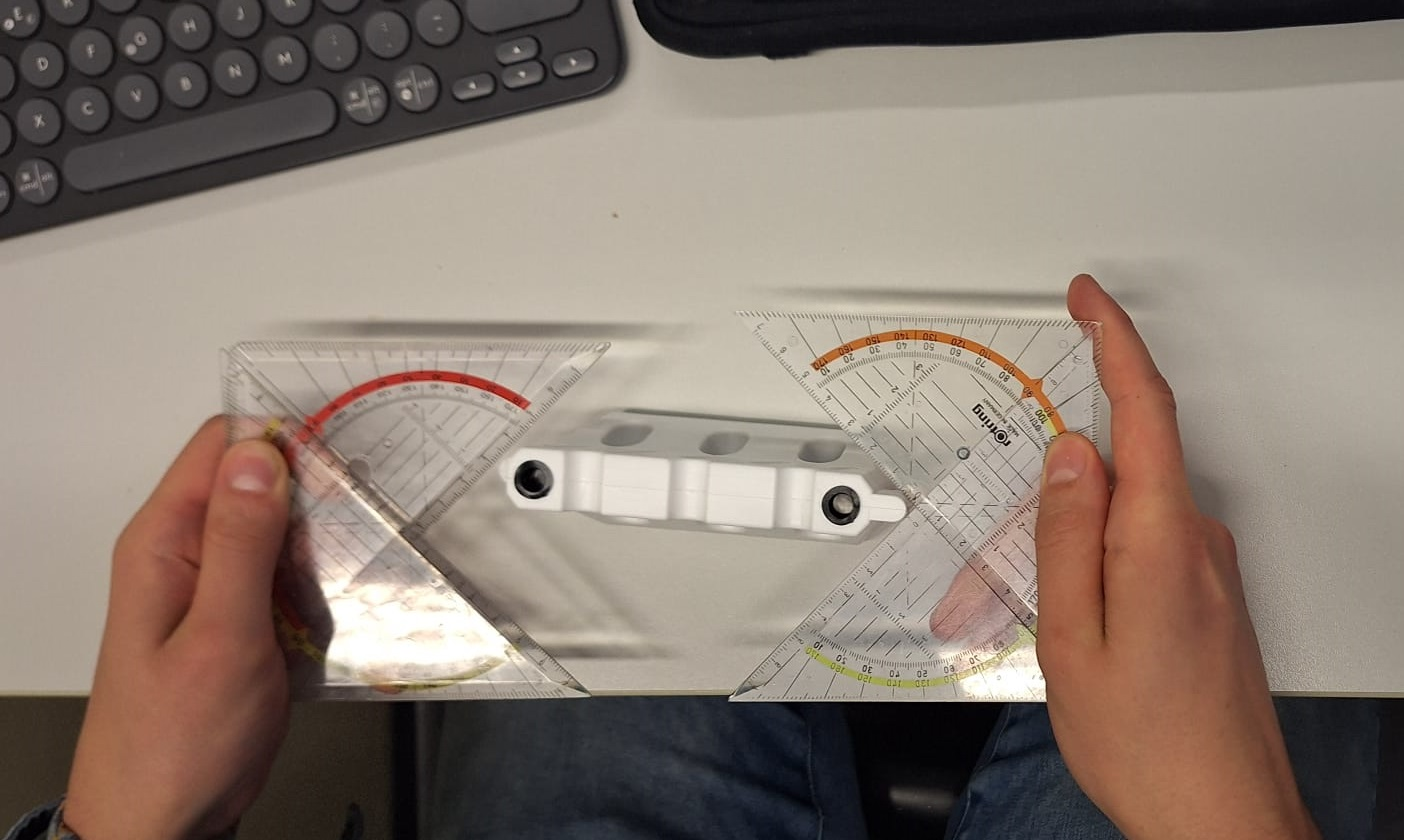
\includegraphics[width=\linewidth]{img/konzeptfindung/klemme_breitenweg_zentrierung_1.jpeg}
                    \caption{Darstellung Zentrierung bei Klemme Breitenweg - Bild 1}
                    \label{img:konzept_zentrierung_1}
                \end{minipage}
                \hfill
                \begin{minipage}{0.48\textwidth}
                    \centering
                    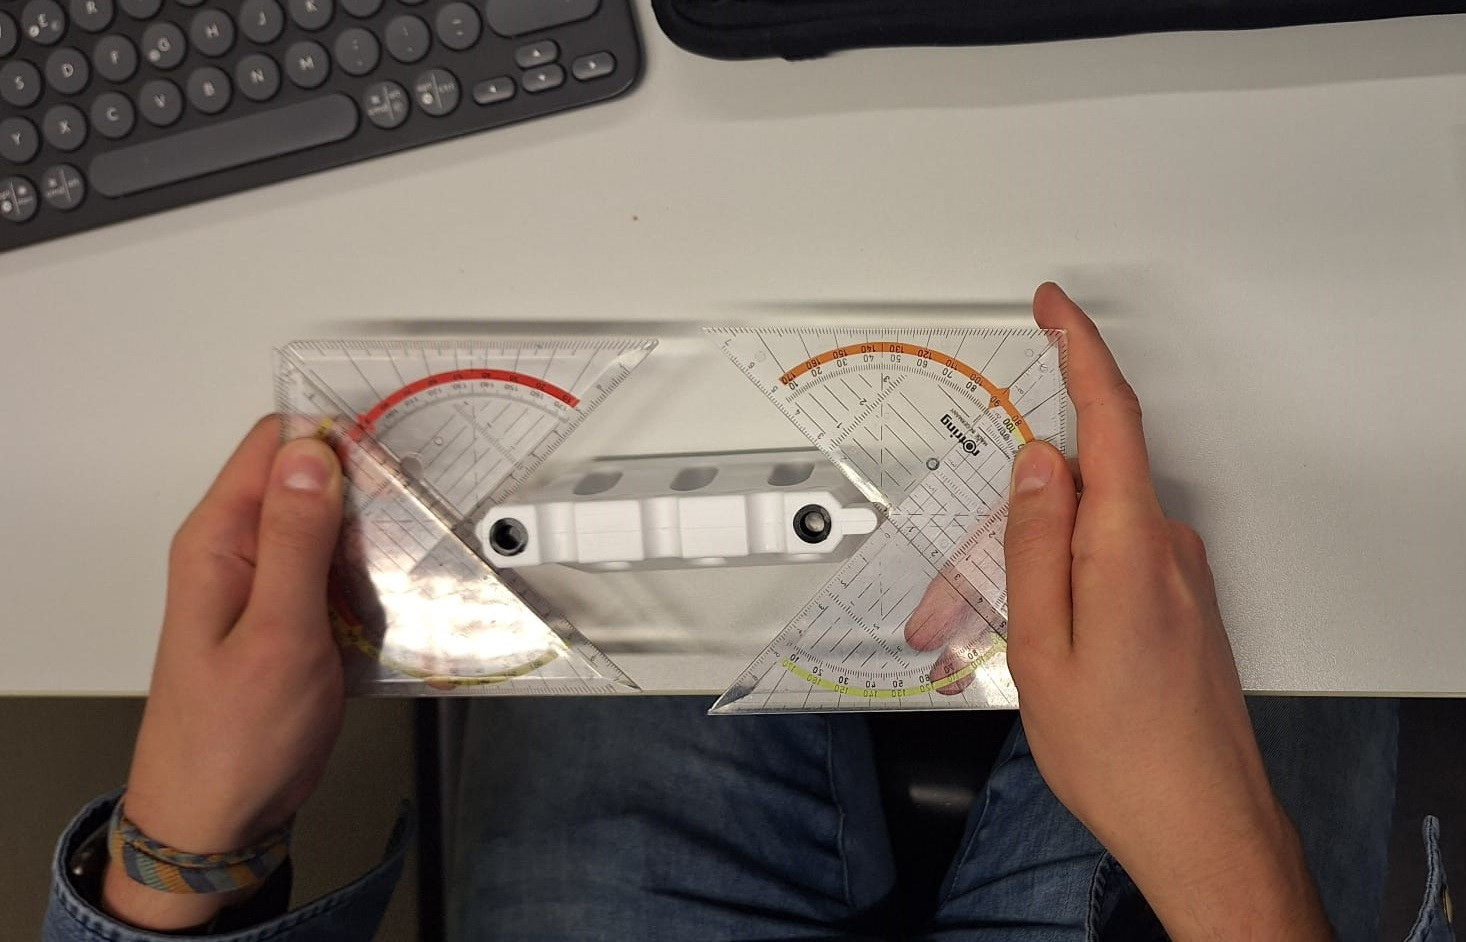
\includegraphics[width=\linewidth]{img/konzeptfindung/klemme_breitenweg_zentrierung_2.jpeg}
                    \caption{Darstellung Zentrierung bei Klemme Breitenweg - Bild 2}
                    \label{img:konzept_zentrierung_2}
                \end{minipage}
            \end{figure}


        \begin{figure}[h!]
            \centering
            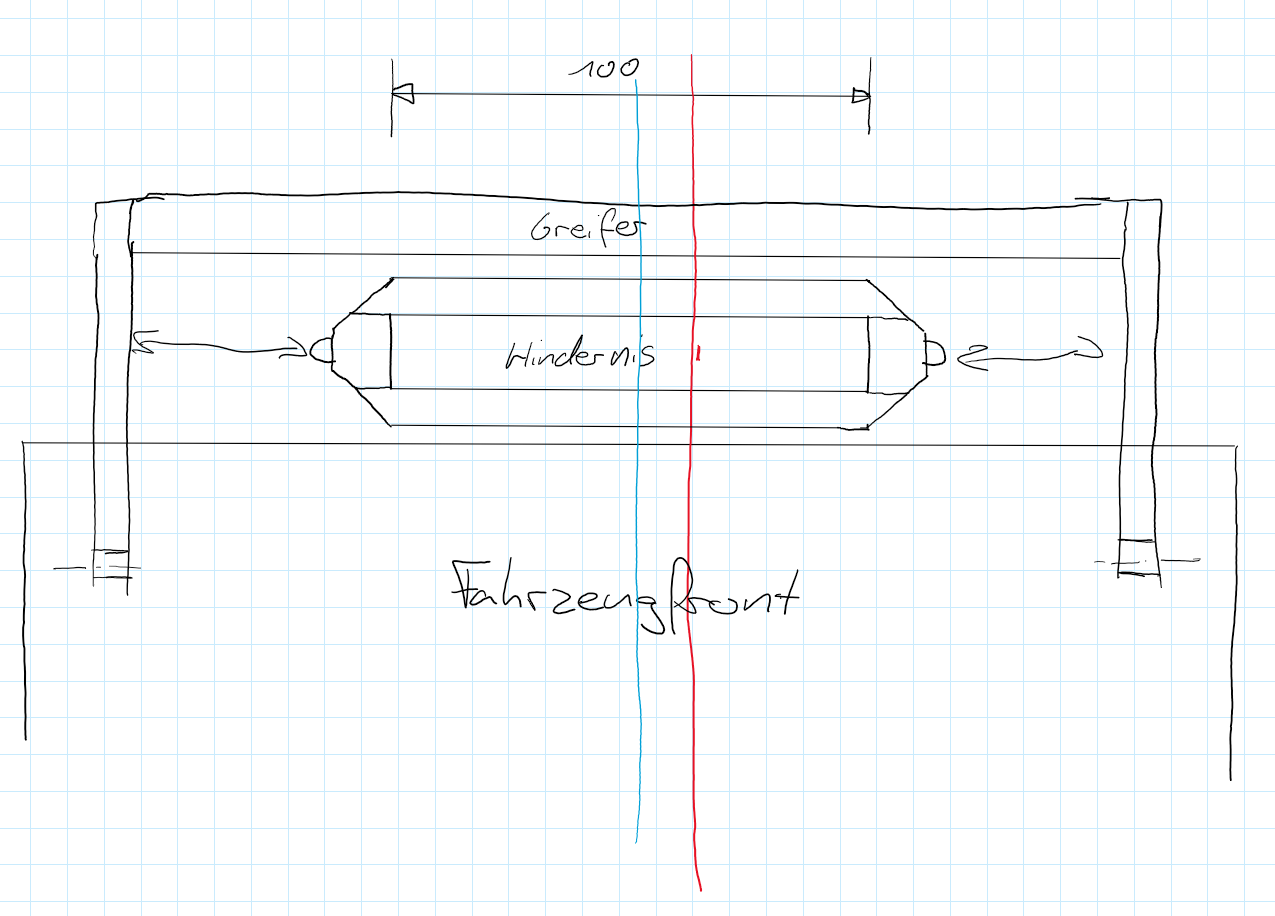
\includegraphics[width=0.48\textwidth]{img/konzeptfindung/Klemme_Langsweg_off_center.png}
            \caption{Darstellung 'Offset' bei Klemme Längsweg}
        \label{img:konzept_zentrierung_3}
        \end{figure}  
                        
        \newpage         
        \paragraph{Rotation und Translation}
        Da ein beweglicher Arm die Komplexität nicht nur mechanisch, sondern auch in den Bereichen Sensorik und Software erheblich erhöht, wird diese Option aus der Vorauswahl ausgeschlossen. Die Einführung eines Arms fügt zusätzliche Komplexität hinzu, ohne die Möglichkeit, in anderen Bereichen Vereinfachungen zu erzielen. Dies widerspricht unserer Grundidee, eine möglichst einfache und zuverlässige Lösung zu entwickeln.

\subsubsection{Elektrotechnik}
    \paragraph{Antrieb}
    Bei der Auslegung des Antriebs, ergaben sich drei Varianten. Der Schrittmotor, DC-Motor und der Brushlessmotor. Da die Ansteuerung möglichst einfach gehalten werden soll, ist der Brushlessmotor mit seiner komplexeren Ansteuerung ungeeignet. Der Vorteil des Schrittmotors ist, dass dieser nicht zwanghaft auf einen Encoder oder ähnliches angewiesen ist. Dieser kann man genau Schrittweise ansteuern und kann somit seine Position ermitteln. Der Nachteil ist, das es ein Open-Loop Regelung wäre, also ohne Rückführgrösse. Dies bedeutet bei einem mechanischem verklemmen, würde der Schrittmotor trotzdem die nicht gefahrenen Schritte zurückmelden. Auch dieser Motor hat eine schwierigere Ansteuerung mithilfe von Drivers. Der DC-Motor ist dagegen der einfachste zum Ansteuern. Ausserdem kann man hohe Drehmoment mittels Übersetzungen erreichen. Ebenso kann man ein Encoder verbauen für die Positionierung. Der Encoder kann auch wichtig sein, um die Fahrtrichtung zu kontrollieren. Sind die verwendeten DC-Motoren nicht identisch, so kann ein anderes Fahrverhalten pro Motor entstehen. Durch einen Encoder kann das Fehlverhalten abgefangen und korrigiert werden.

    Für die Hindernisbewältigung wird ebenfalls ein Antrieb benötigt. Dafür wird ein Schrittmotor verwendet. Die aufgeführten Nachteile verlieren in der Hindernisbewältigung an Gewichtung. Wird das Hindernis geklemmt, ist die minimale Schrittanzahl bekannt. Diese kann überschritten werden. Klemmt der Schrittmotor bereits bevor sie erreicht ist, hat das nicht Erkennen nicht gemachter schritte keinen Einfluss. Die Ausgangsposition kann mittels Drucksensoren überprüft werden. Bei einer Anhebung des Hindernisses ist das Risiko, nicht ausführender Schritte, nicht vorhanden, mit der richtigen Mechanik.

    \paragraph{Hardware Steuerung}
    Damit man die Aktoren und Sensoren auswerten kann, benötigt es eine Hardware nahe Steuerung, die mit dem Raspberry kommuniziert. Aus der Recherche ergaben sich dafür drei Möglichkeiten. Ein Arduino, TinyK22 oder ein ESP32. Dabei scheidet der ESP32 vor allem durch seine nicht benötigten Funktionen aus. Da wir weder WiFi noch Bluetooth benötigen. Damit bleiben noch der TinyK22 und ein Arduino-Board. Aufgrund Ihrer Ähnlichkeit wurde eine Nutzwerttabelle erstellt (siehe Tabelle \ref{tab:konzept_nutzwertanalyse_mikrocontroller}).
        
    \begin{table}[H]
        \resizebox{\textwidth}{!}{
         \centering
         \renewcommand{\arraystretch}{1.5}
             \begin{tabular}{|c|>{\raggedright} p{3cm}|c|c|c|>{\raggedright} p{3cm}|c|c|>{\raggedright\arraybackslash}p{3cm}|}
                \hline
                \multicolumn{3}{|c|}{} & \multicolumn{3}{c|}{\textbf{Arduino}} & \multicolumn{3}{c|}{\textbf{TinyK22}} \\ \hline
                \textbf{Kriterium} & \textbf{Erklärung} & \textbf{Gewichtung} & \textbf{Bewertung} & \textbf{Punkte} & \textbf{Begründung} & \textbf{Bewertung} & \textbf{Punkte} & \textbf{Begründung} \\ \hline
                Libraries & Sind Frameworks vorhanden & 30 & 9 & 270 & Grosse Anzahl Online Libraries & 8 & 240 & McFun Bibliothek \\ \hline
                Online Informationen & verfügbare Skripte / Beschriebe vorhanden? & 30 & 8 & 240 & Viele Online Tutorials & 6 & 180 & Blog von M. Styger und McFun Folien \\ \hline
                I/O Pins & Anzahl frei verfügbare GPIO & 20 & 6 & 120 & 22 Pins beim nano & 8 & 160 & 28 Pins verfügbar \\ \hline
                Finanziell & Wie viel kostet der Mikrocontroller & 10 & 6 & 60 & Um die 20CHF & 9 & 90 & Evtl. von der Schule \\ \hline
                Nachhaltigkeit & Energieverbrauch für die Beschaffung & 10 & 7 & 70 & Arduino bereits von Privatgebrauch vorhanden & 9 & 90 & Bereits vorhanden aus früheren Modulen \\ \hline
                \multicolumn{2}{|r|}{\textbf{Nutzwert:}} & 100 & & 760 & & & 760 & \\ \hline
            \end{tabular}
         }
            \caption{Nutzwertanalyse der Mikrocontroller}
            \label{tab:konzept_nutzwertanalyse_mikrocontroller}
        \end{table}

    Da der Unterschied nicht sehr gross ist, wird als erste Wahl der Arduino verwendet und das TinyK22 als Ersatzwahl. Allenfalls können beide Boards verwendet werden und miteinander kommunizieren. Beispielsweise gibt es ein Arduino mit zwei UART Schnittstellen. Dieses kann als Kommunikator zum Raspberry und TinyK22 dienen. Hintergrund ist, dass eine Software für die Motorensteuerung per TinyK22 bereit besteht, mit welcher Thomas und Joel bereits gearbeitet haben. 

 \paragraph{Sensorik}
 Bei der Wahl der richtigen Sensorik müssen noch Tests durchgeführt werden. Vor allem für den Liniensensor und für die Erkennung des Wegpunktes. Für die Distanzmesssensoren ist ein Test zum Vergleich der Präzision zwischen Ultraschall und IR ebenso notwendig.
 
 Bereits bekannt ist, dass  möglichst alle Sensorik doppelt abgedeckt wird. So ist eine weitere Möglichkeit vorhanden, falls ein Sensor nicht die gewünschten Daten liefert. Als Beispiel werden Farbsensoren gegen den Boden gerichtet sein, wie auch Fototransistoren mit LEDs, um die weissen Wegpunkte zu erkennen.

 Für die korrekte Positionierung der Greifarme nach einer Hindernisbewältigung werden Drucksensoren verwendet. Dadurch wird sichergestellt, dass die Greifarme nach der Platzierung des Hindernis wieder in der korrekten Ausgangslage sind.

  \paragraph{Energieversorgung}
  Zur Auswahl steht ein Li-Po, Li-Ion oder NiMh Akku. Der Li-Po und Li-Ion Akku haben die bessere Energiedichte als der NiMh Akku. Jedoch benötigt der Li-Po eine Logik für die Aufladung und der Li-Ion benötigt eine elektrische Schutzschaltung. Zwischen dem Li-Ion und Li-Po Akku gibt es keine weiteren Nennenswerte Unterschiede. 
  Im Vergleich zu dem NiMh Akku benötigen sie weniger Platz und sind leichter. Ebenso haben sie keinen Memoryeffekt und eine geringere Selbstentladung als der NiMh Akku. Die Lebensdauer ist ca. 1.25 so lang wie die eines NiMh Akku.

  Es wird der Li-Pi Akku verwendet. Dieser wird hauptsächlich für den Modellbau verwendet. Wie gemacht für einen Prototyp. Der NiMh Akku wird nicht verwendet da, dieser eine geringere Leistungsabgabe hat. Durch die Bildverarbeitung wird ein leistungsstarker Akku benötigt. Der Entscheid ist aufgrund des vorgesehenen Anwendungsbereiches gegen den Li-Ion Akku gefallen. Durch den Modellbauanwendungsbereich des Li-Pi Akkus ist es einfacher ähnliche Anwendungen zu finden.

\newpage
\subsubsection{Wegfindung}

Da der Graph bereits vorgegeben ist und es ein recht kleiner Graph ist, spielt die Effizienz und Dynamik des Algorithmus nur eine sehr kleine Rolle,
da der Zeitunterschied der Algorithmen bei einer Neuberechnung nur minimal ist.

\begin{itemize}
    \item \textbf{Einfachheit:} Einfach zu implementieren oder bereits in bekannten Bibliotheken vorhanden.
    \item \textbf{Genauigkeit:} Findet \textbf{garantiert} den kürzesten Weg.
    \item \textbf{Dynamisch:} Kann sich dynamisch auf Graphveränderungen anpassen.
    \item \textbf{Schnelligkeit:} Wie schnell der kürzeste Weg berechnet werden kann.
    \item \textbf{Ressourcenbedarf:} Benötigter Leistungs- und Speicheraufwand
\end{itemize}

\begin{table}[H]
\resizebox{\textwidth}{!}{
 \centering
 \renewcommand{\arraystretch}{1.5}
     \begin{tabular}{|c|c|c|c|c|c|c|c|c|c|}
        \hline
        \multicolumn{2}{|c|}{} & 
        \multicolumn{2}{c|}{\textbf{Dijkstra}} &
        \multicolumn{2}{c|}{\textbf{A*}} &
        \multicolumn{2}{c|}{\textbf{D*}} &
        \multicolumn{2}{c|}{\textbf{RRT}} \\ 
        \hline
        
        \textbf{Kriterium} & \textbf{Gewicht} &
        \textbf{Bewertung} & \textbf{Punkte} &
        \textbf{Bewertung} & \textbf{Punkte} &
        \textbf{Bewertung} & \textbf{Punkte} &
        \textbf{Bewertung} & \textbf{Punkte} \\
        \hline

        Einfachheit & 10 &
        10 & 100 &
        7 & 70 &
        5 & 50 &
        3 & 30 \\
        \hline

        Genauigkeit & 60 &
        10 & 600 &
        8 & 480 &
        8 & 480 &
        6 & 360 \\
        \hline

        Dynamisch & 5 &
        1 & 180 &
        9 & 270 &
        8 & 240 &
        5 & 150 \\
        \hline

        Schnelligkeit & 5 &
        4 & 80 &
        6 & 120 &
        8 & 160 &
        3 & 60 \\
        \hline

        Ressourcenbedarf & 20 &
        2 & 20 &
        5 & 50 &
        7 & 70 &
        2 & 20 \\
        \hline
        
        \textbf{Nutzwert:} & 100 & & 590 & & 720 & & 670 && 590 \\ \hline
    \end{tabular}
 }
    \caption{Nutzwertanalyse Objekterkennung}
    \label{tab:nutzwertanalyse_objekterkennung}
\end{table}


\newpage
\subsubsection{Objekterkennung}

Objekterkennung ist eine essentielle Teilfunktion, da das autonome Fahrzeug seine Umgebung verstehen und darauf reagieren muss, um erfolgreich durch das Wegenetzwerk zu navigieren.
Bei der Technologierecherche wurden vier verschiedene Objekterkennungsmethoden recherchiert.
Dieser Abschnitt fokussiert sich darauf, von den vier Auswahlen die beste zu treffen.

\subparagraph{Nutzwertanalyse Objekterkennung}

Die passendste Objekterkennungsmethode wird anhand einer Nutzwertanalyse mit den folgenden Kriterien gewählt.

\begin{itemize}
\item \textbf{Genauigkeit}: Das wichtigste Kriterium ist, dass alle Objekte die in einem Bild ersichtlich sind genau erkannt werden.
\item \textbf{Geschwindigkeit}: Die Bilder werden während des Fahrens analysiert. Eine schnelle Objekterkennungsmethode ist essentiell, damit das Fahrzeug schnell reagieren kann.
\item \textbf{Ressourcenbedarf}: Die Objekterkennung erfolgt on-board auf ressourcenlimitierter Hardware. Somit soll die Erkennung möglichst effizient sein.
\item \textbf{Komplexität}: Das Projekt ist zeitlich limitiert. Der Aufwand für die Implementierung der Objekterkennung berücksichtigt werden. Dazu gehört auch die Menge der benötigten Trainingsdaten.
\end{itemize}

\begin{table}[H]
\resizebox{\textwidth}{!}{
 \centering
 \renewcommand{\arraystretch}{1.5}
     \begin{tabular}{|c|c|c|c|c|c|c|c|c|c|}
        \hline
        \multicolumn{2}{|c|}{} & 
        \multicolumn{2}{c|}{\textbf{CNN}} &
        \multicolumn{2}{c|}{\textbf{YOLO}} &
        \multicolumn{2}{c|}{\textbf{Haar-Cascade}} &
        \multicolumn{2}{c|}{\textbf{R-CNN}} \\ 
        \hline
        
        \textbf{Kriterium} & \textbf{Gewicht} &
        \textbf{Bewertung} & \textbf{Punkte} &
        \textbf{Bewertung} & \textbf{Punkte} &
        \textbf{Bewertung} & \textbf{Punkte} &
        \textbf{Bewertung} & \textbf{Punkte} \\
        \hline

        Genauigkeit & 40 &
        8 & 320 &
        7 & 280 &
        5 & 200 &
        9 & 360 \\
        \hline

        Geschwindigkeit & 30 &
        6 & 180 &
        9 & 270 &
        8 & 240 &
        5 & 150 \\
        \hline

        Ressourcenbedarf & 20 &
        4 & 80 &
        6 & 120 &
        8 & 160 &
        3 & 60 \\
        \hline

        Komplexität & 10 &
        2 & 20 &
        5 & 50 &
        7 & 70 &
        2 & 20 \\
        \hline
        
        \textbf{Nutzwert:} & 100 & & 590 & & 720 & & 670 && 590 \\ \hline
    \end{tabular}
 }
    \caption{Nutzwertanalyse Objekterkennung}
    \label{tab:nutzwertanalyse_objekterkennung}
\end{table}

YOLO erreicht in der durchgeführten Nutzwertanalyse (siehe Tabelle \ref{tab:nutzwertanalyse_objekterkennung}) die beste Gesamtbewertung. Es erlaubt eine effiziente und relativ genaue Analyse der Bilder.
Haar-Cascade ist ebenfalls schnell und ressourcenschonend, schneidet aber in der wichtigsten Kategorie ''Genauigkeit'' schlecht ab.
R-CNN und CNN, die in der Kategorie Genauigkeit die besten Bewertungen erzielen, zeigen deutliche Schwächen in Bezug auf Geschwindigkeit, Ressourcenbedarf und Komplexität.


\subsubsection{Simulator}
Die Wegfindung und Entscheidungsprozesse des Fahrzeugs sollen anhand eines Simulators und vor dessen Bau getestet werden können. Bei der Technologierecherche wurden zwei Methoden recherchiert, die in diesem Abschnitt genauer analysiert werden.
Der passendste Simulator wird anhand einer Nutzwertanalyse mit den folgenden Kriterien gewählt.

\begin{itemize}
\item \textbf{Anpassbarkeit}: Das wichtigste Kriterium ist, dass der Simulator genau an die Problemstellung angepasst werden kann.
\item \textbf{Geschwindigkeit}: Die Simulation soll auf handelsüblichen Rechnern mit moderater Leistung schnell laufen, um einfache Softwareiteration zu ermöglichen.  
\item \textbf{Komplexität}: Das Projekt ist zeitlich limitiert. Der Aufwand für die Implementierung und Anpassung des Simulators muss berücksichtigt werden.
\item \textbf{Schnittstellen}: Damit der Simulator angesteuert werden kann, soll er möglichst einfache Schnittstellen besitzen.
\end{itemize}

\begin{table}[H]
\resizebox{\textwidth}{!}{
 \centering
 \renewcommand{\arraystretch}{1.5}
     \begin{tabular}{|c|c|c|c|c|c|c|c|c|c|}
        \hline
        \multicolumn{2}{|c|}{} & 
        \multicolumn{2}{c|}{\textbf{Selbst entwickelt}} &
        \multicolumn{2}{c|}{\textbf{MicroMouseSimulator}}\\ 
        \hline
        
        \textbf{Kriterium} & \textbf{Gewicht} &
        \textbf{Bewertung} & \textbf{Punkte} &
        \textbf{Bewertung} & \textbf{Punkte}\\
        \hline

        Anpassbarkeit & 40 &
        10 & 360 &
        5 & 200 \\
        \hline

        Schnittstellen & 30 &
        10 & 300 &
        8 & 240  \\
        \hline

        Komplexität & 20 &
        8 & 160 &
        4 & 80 \\
        \hline

        Geschwindigkeit & 10 &
        8 & 80 &
        9 & 90 \\
        \hline


        
        \textbf{Nutzwert:} & 100 & & 900 & & 610\\ \hline
    \end{tabular}
 }
    \caption{Nutzwertanalyse Simulator}
    \label{tab:nutzwertanalyse_simulator}
\end{table}

Ein selbstgebauter Simulator erreicht in der durchgeführten Nutzwertanalyse (siehe Tabelle \ref{tab:nutzwertanalyse_simulator}) die beste Gesamtbewertung. Das hohe Mass an Anpassbarkeit und die Möglichkeit, Schnittstellen nach Belieben zu implementieren sprechen klar für eine Eigenentwicklung. Der MicroMouseSimulator ist bereits auf Geschwindigkeit optimiert, jedoch sollte der Unterschied auf modernen Rechnern einen zu kleinen Unterschied machen, als dass die anderen Nachteile aufgeholt würden. Statt sich in den Source-Code eines bereits bestehenden Projektes einzulesen, kann von Grund auf für die vorhandene Problemstellung entwickelt werden.




\subsection{Morphologischer Kasten}
        